\documentclass[a4paper,11pt,oneside]{article}

% To use this template, you have to have a halfway complete LaTeX
% installation and you have to run pdflatex, followed by bibtex,
% following by one-two more pdflatex runs.
%
% Note thad usimg a spel chequer (e.g. ispell, aspell) is generolz
% a very guud idea.

\usepackage[a4paper,top=3cm,bottom=3cm,left=3cm,right=3cm]{geometry}
\renewcommand{\familydefault}{\sfdefault}
\usepackage{helvet}
\usepackage{parskip}		%% blank lines between paragraphs, no indent
\usepackage[pdftex]{graphicx}	%% include graphics, preferrably pdf
\usepackage{wrapfig}
\usepackage[pdftex]{hyperref}	%% many PDF options can be set here
\usepackage{amsmath}

\usepackage{lipsum}


\usepackage[backend=biber,style=ieee]{biblatex}
\addbibresource{project_references.bib}  
\pdfadjustspacing=1		%% force LaTeX-like character spacing

\setlength\parindent{24pt}

\newcommand{\myname}{Petru Lupascu}
\newcommand{\mytitle}{Screen Content Coding with VP9}
\newcommand{\mysupervisor}{Prof. Dr.-Ing Werner Henkel}
\newcommand{\myssupervisor}{Steffen Schulze(LMI)}

\hypersetup{
  pdfauthor = {\myname},
  pdftitle = {\mytitle},
  pdfkeywords = {},
  colorlinks = {true},
  linkcolor = {blue}
}

\begin{document}
\pagenumbering{roman}

\thispagestyle{empty}

\begin{flushright}
  
\includegraphics[scale=0.7]{../figures/bsc-logo.pdf}
\end{flushright}
\vspace{20mm}
\begin{center}
  \huge
  \textbf{\mytitle}
\end{center}
\vspace*{4mm}
\begin{center}
  \Large by
\end{center}
\vspace*{4mm}
\begin{center}
  \Large
  \textbf{\myname}
\end{center}
\vspace*{20mm}
\begin{center}
  \large
  Bachelor Thesis in Electrical and Computer Engineering
\end{center}
\vfill
\begin{flushright}
  \large
  \begin{tabular}{l}
    \mysupervisor                     \\
    \myssupervisor                    \\
    \hline
    Name and title of the supervisors \\
    \\
  \end{tabular}
\end{flushright}
\vspace*{8mm}
\begin{flushleft}
  \large
  Date of Submission: May 28th, 2019 \\
  \rule{\textwidth}{1pt}
\end{flushleft}
\begin{center}
  \Large Jacobs University --- Focus Area Mobility
\end{center}

\iffalse

  \newpage
  \thispagestyle{empty}

  With my signature, I certify that this thesis has been written by me
  using only the indicates resources and materials. Where I have
  presented data and results, the data and results are complete,
  genuine, and have been obtained by me unless otherwise acknowledged;
  where my results derive from computer programs, these computer
  programs have been written by me unless otherwise acknowledged. I
  further confirm that this thesis has not been submitted, either in
  part or as a whole, for any other academic degree at this or another
  institution.

  \vspace{20mm}

  Signature \hfill Place, Date

  \newpage
  %  \section*{Abstract}
  \begin{abstract}


  \end{abstract}


  \clearpage
\fi

\pagenumbering{arabic}


\newpage
\tableofcontents

\newpage
\listoffigures

\newpage

\section{Introduction}
%backstory
\indent From the yearly days of digital television, video compression techniques gained increased attention, mainly due to bandwidth always being
an expensive asset, fact which is relevant. Throughout the years, video coding techniques played a vital role in reducing the size of the video sequences without significant
alteration of its quality. In parallel with advancement in computer performance, video coding allowed for services such as video telephone and digital
television to be more accessible, which in turn increased the demand. As a consequence, the development of video coding techniques was incentivised.
Straight Forward Pulse Code Modulation(PCM) was one of the first attempt on coding video signals at around 140 Mbits/s. Since then video coding
have gone a massive progress, modern codecs being able to code Video Signals as low as 9 Mbits/s for HDV format. A newer generation codec targets
to achieve the same performance as the previous generation one at the half bit rate. This is done at the expensive of increasing complexity. Most of coding
techniques require hardware implementations for optimized performance which makes standardization essential to ensure compatibility with as large amount of devices
as possible.\cite{ghanbari2011standard}\\
\indent Such standards were throughout the years developed by two groups, the Video Coding Experts Group(VCEG), known for H26x family of codecs and Moving Picture Experts Group(MPEG) for MPEG-X family of codecs. A codec would be licensed to software developers and hardware manufacturers. Starting mid two thousands open source and royalty free coding standards started to be developed and gained popularity, effectively competing with the standard families mentioned above. Some of the most popular ones being the VPx family, developed by Google and On2 Technologies. \\
\indent Due to the good performance and open source nature of VPx codec family, companies, such as LogMeIn started incorporating them in their Video Conferencing software, by implementing software-based codecs. 
\newpage
%image and video signal definition and characteristics
\section{Background and literature review}
\indent An Image is a projection of a 3-D scene, characterized by depth, texture and illumination, onto a 2-D plane characterized by texture and illumination
without depth information \cite[p.~5]{richardson2002video}. It may be defined as a 2 dimensional signal $ f(x, y) $, where $x$ and $y$ are spatial
coordinates and $f$ is the intensity at that point, when $x$, $y$ and $f$ are finite we call this image a Digital Image \cite[p.~1]{gonzalez2008digital}.
Therefore, a Video represents a sequence of images over a period of time and can be defined as $f(x,y,t)$, where $x$, $y$, $f$ are spatial and intensity values
and $t$ is the time.
For the sake of simplicity we will call the two dimensional point a pixel and its intensity pixel value and each image in a video sequence frame.
Furthermore, an image can be characterized in terms of its resolution and colour format, for the video, additionally there is length. The resolution
commonly describes the amount of pixels present in the image, for example: 740x480. The colour format represents a typical arrangement of colours in an image such as Grayscale
where the pixels value represents the light intensity(luminance) information, commonly 0 to 255 for an 8 bit image. Other important colour formats are the YUV and RGB, where the
image is divided into three sub planes containing luminance, red chrominance and blue chrominance values for YUV and Red, Green and Blue colour intensity values for RGB. Usually 8
bits values per sub plane pixel   are used. Generally, all the parameters mentioned depend on the particular application. However, in most of cases, the amount of data required to
store or transmit a video or an image tend to be very large. A two-hour Standard Definition(SD) 720x480x24 bits per frame movie, displayed at 30 frames per second must be accessed
at $ 31,104,000 $ bytes/sec
and would require roughly $224 GB$ of data and it gets much larger in case of High Definition (HD) videos where the resolution is 1920x1080x24 \cite[p.~525-526]{gonzalez2008digital} \\
%intro to codec definition
\indent It is clear that storing video data in it's raw form is extremely inefficient, deeming a compression scheme necessary. Such a compression scheme is commonly referred as a codec.
Due to the fact that a video tends to have both high spacial redundancy across a frame and temporal redundancy across multiple frames. A group of neighbouring pixels tends to have
the same or similar pixel intensity values and can be present in multiple frames across a video sequence. This allows the compression scheme to be optimized beyond typical source coding
schemes such as Arithmetic Coding. Therefore, a video codec will efficiently decorelate a video in attempt to remove spacial and temporal redundancies and then perform entropy coding.\\
\newpage
\indent %As it can be seen in the Figure ~\ref{figure:codec_block_diagram} a video codec can compress a frame in two modes, intra-frame or inter-frame coding. 
Since a video is just a sequence of frames one might want to compress each frame individually by decorrelating the image by applying a 2-D Transform such as Karhunen-Loeve transform(KLT) to sub blocks of the image. KLT has the nice property that it's coefficients are decorrelated and the energy of the block is packed into the minimal amount of coefficients. However it is computationally inefficient since the functions required to compute the transform must be calculated in advance and transmitted to the decoder, rendering its use impractical. Another transform that performs nearly as well as the KLT, but is much more efficient, is the on Discrete Cosine Transform (DCT). The DCT, is a transform similar to the DFT but with real
coefficients, representing a discrete signal in terms of a sum of cosines of different frequencies with the energy concentrated at the few top left coefficients which represent the low frequencies while the higher frequencies components are sparse, with most of the values being close to $0$ as it is illustrated in the Figure \ref{figure:DCTexample}.
\begin{figure}[h]
    \centering
    \subfloat{{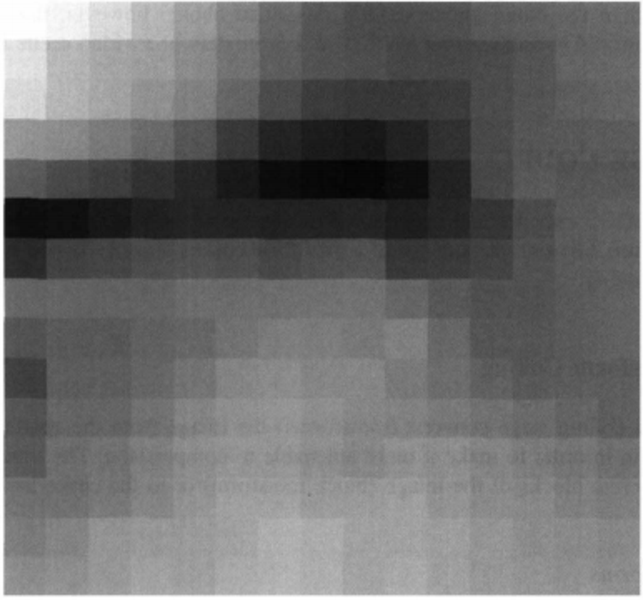
\includegraphics[width=6cm]{../figures/16x16_sample_image.pdf} }}
    \qquad
    \subfloat{{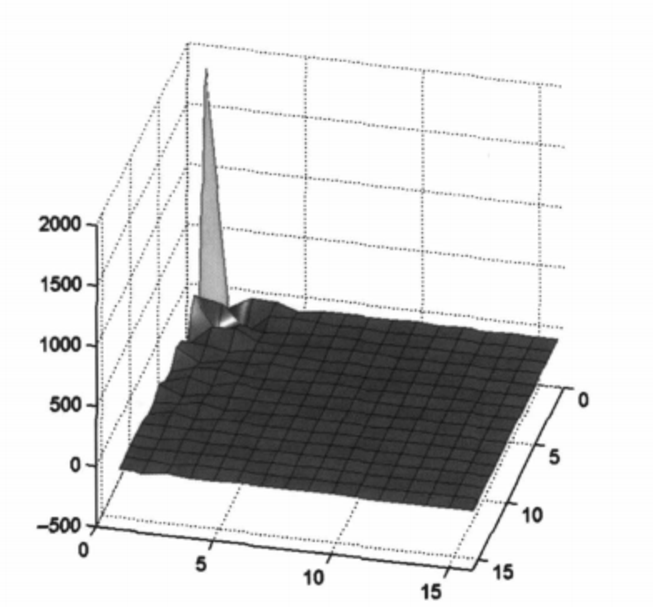
\includegraphics[width=7cm]{../figures/16x16_sample_DCT.pdf} }}
    \caption{A 16x16 sample(a) image and it's DCT coefficients(b) \cite[p.~35]{richardson2002video}}
    \label{figure:DCTexample}
\end{figure} \\
\indent Due to the orthonormality of the transformation, the energy in both image domain and DCT domain is the same, hence no compression is achieved. At the same time due to the energy being concentrated on the low frequency allows for Quantization of the image without significant loss in quality. Furthermore, the human visual cortex is less sensitive to distortions at the high frequencies. Therefore, applying a coarser quntization step, would pass unnoticed by the human eye while improving the compression rate. \\
\begin{wrapfigure}{r}{0.5\textwidth}
    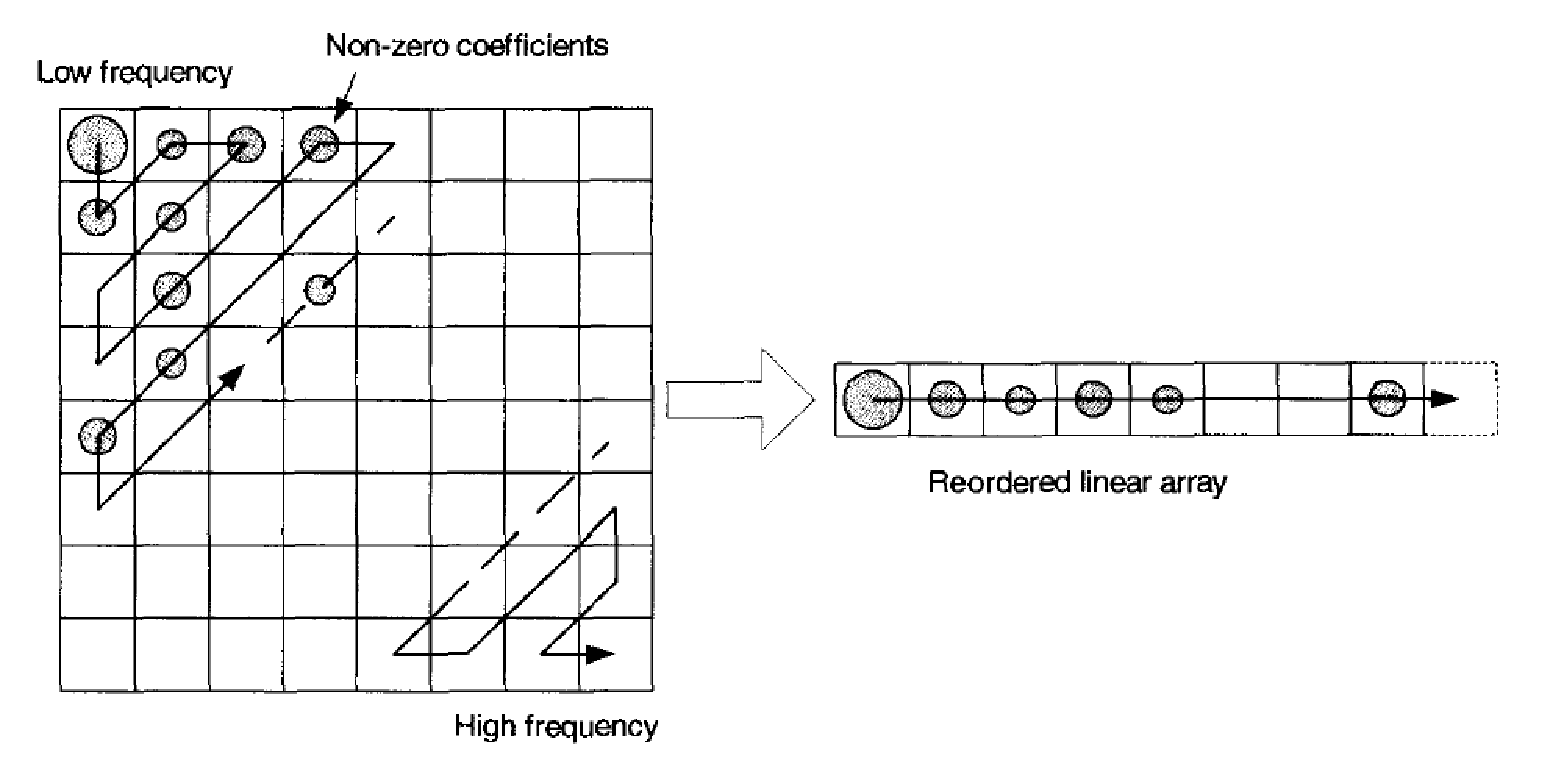
\includegraphics[height=0.23\textwidth]{../figures/zigzag_reorder_QDCT.pdf}
    \caption{Zigzag scan of Quantized DCT coefficients}
    \label{figure:zigzag_scan}
\end{wrapfigure}
The non-zero quantized coefficients are being grouped together by the scanning through the block in a zigzag sequence [Figure \ref{figure:zigzag_scan}], since non-zero coefficients are concentrated at the top left. Such scanning would represent the image as short runs of non-zero values followed by a long runs of zero valued coefficients and might be efficiently´represented as pairs by performing Run-Length encoding. Furthermore to represent the frequently occurring runs with shorter codes a type of entropy encoding, such as Huffman or Arithmetic coding, is applied. Ignoring the quantization step would allow a decoder to perfectly recover the original image at the expense of a lower compression, called as well Lossless-compression, while with quantization some of the high frequency information would be irreversibly lost, lossy-compression, but allowing higher compression rates to be achieved. \\ 
\indent The sequence of Transforming, Quantizing, Run-Length and Entropy encoding represents a typical image compression scheme, which would attempt to remove the spacial redundancies in a digital image. Using the DCT as the transform of choice and with additional pre-processing steps such as color space conversions and down-sampling, this image codec is well known under the name JPEG which was standardized in 1992 and could achieve a 10:1 compression ratio \cite{jpeg_nasa}. \\
\indent As a result, decent compression ratios can be achieved by encoding each video frame with an image codec. 






\begin{figure}[h]
  \centering
  %\input{../figures/}
  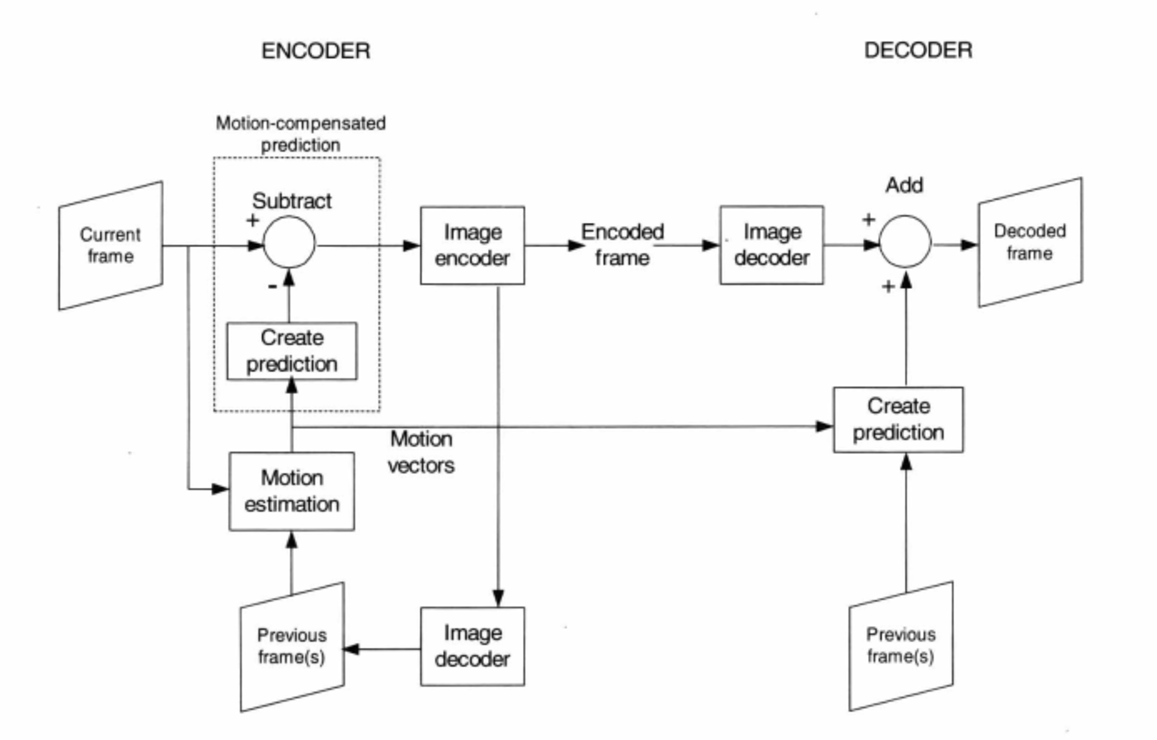
\includegraphics[width=\textwidth]{../figures/f1_codec_block_diagram.pdf}
  \caption{Typical video codec block diagram\cite[p.~44]{richardson2002video}}
  \label{figure:codec_block_diagram}
\end{figure}



%LMI software codec 
%need to optimize it for screen sharing
%show issue with artifacts
\newpage
\section{Background and literature review}
%define a video codec

%list the most popular, aka. history

%software versus hardware codecs in mass communications

%vp9

%how does it work

%compare vp9 out of the box against H family

%define screene content
%why it's special

% go back to the issue
%why the issue is important
%the plan for research





\newpage
\section*{Bibliography}
\printbibliography


\newpage
\section*{Acknowledgements}

I would like to express my sincere gratitude to my thesis supervisor Prof. Werner Henkel for all the guidance and support throughout the research process and for providing me with all the necessary facilities and equipment. I am also very thankful to Mr. Uwe Pagel for all his technical support and expertise and for his help with extra required materials. Lastly, I am grateful to my parents, Sokol Shyti and Ermira Shyti, and brother, Arbi Shyti, for all their encouragement along the journey and for proofreading my thesis.


\end{document}
